\documentclass[10pt]{beamer}
\usepackage{uglixbeamer}
\title{Fonctions}
\author{NSI1}

\begin{document}
	\maketitle
    \section{Exemples de fonctions}
    \begin{frame}{Un objet déjà connu}
        Nous avons déjà rencontré des fonctions \alert{côté utilisateur}:\pause
        \begin{itemize}
            \item \mintinline{python}{input} \pause
            \begin{itemize}
                \item prend en entrée une chaîne de caractères;\pause
                \item renvoie la chaîne de caractère saisie par l'utilisateur.\pause
            \end{itemize}
            On peut noter ceci \mintinline{python}{input(chaine : str) -> str}\pause
            \item \mintinline{python}{len}\pause
            \begin{itemize}
                \item	prend en entrée une liste;\pause
                \item	renvoie le nombre d'éléments de cette liste.\pause
            \end{itemize}
            On peut noter cela \mintinline{python}{len(L : list) -> int}
        \end{itemize}
    \end{frame}

    \begin{frame}{De multiples formes}
        Les deux exemples précédents rentrent dans cette catégorie :
        \begin{center}
            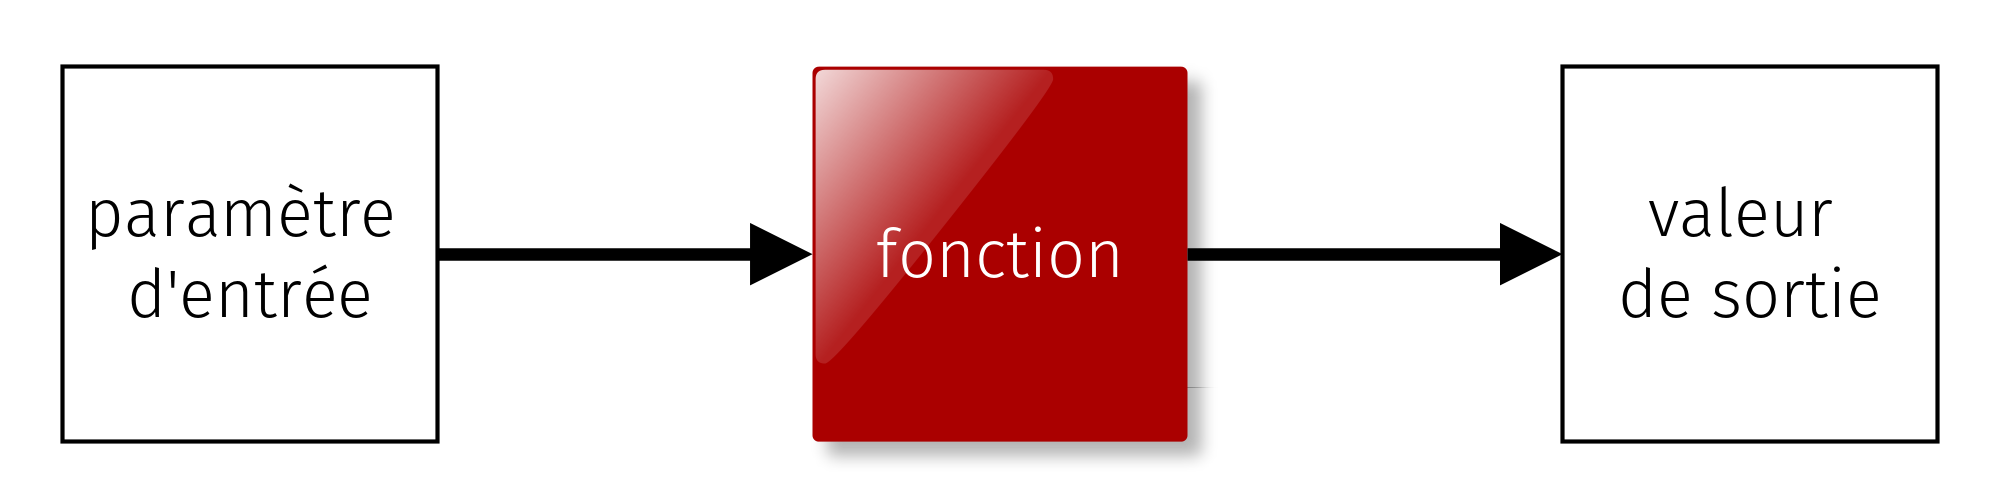
\includegraphics[width=6cm]{img/fonction1.png}
        \end{center}
    \end{frame}
    \begin{frame}{De multiples formes}
        Certaines fonctions sont ainsi :
        \begin{center}
            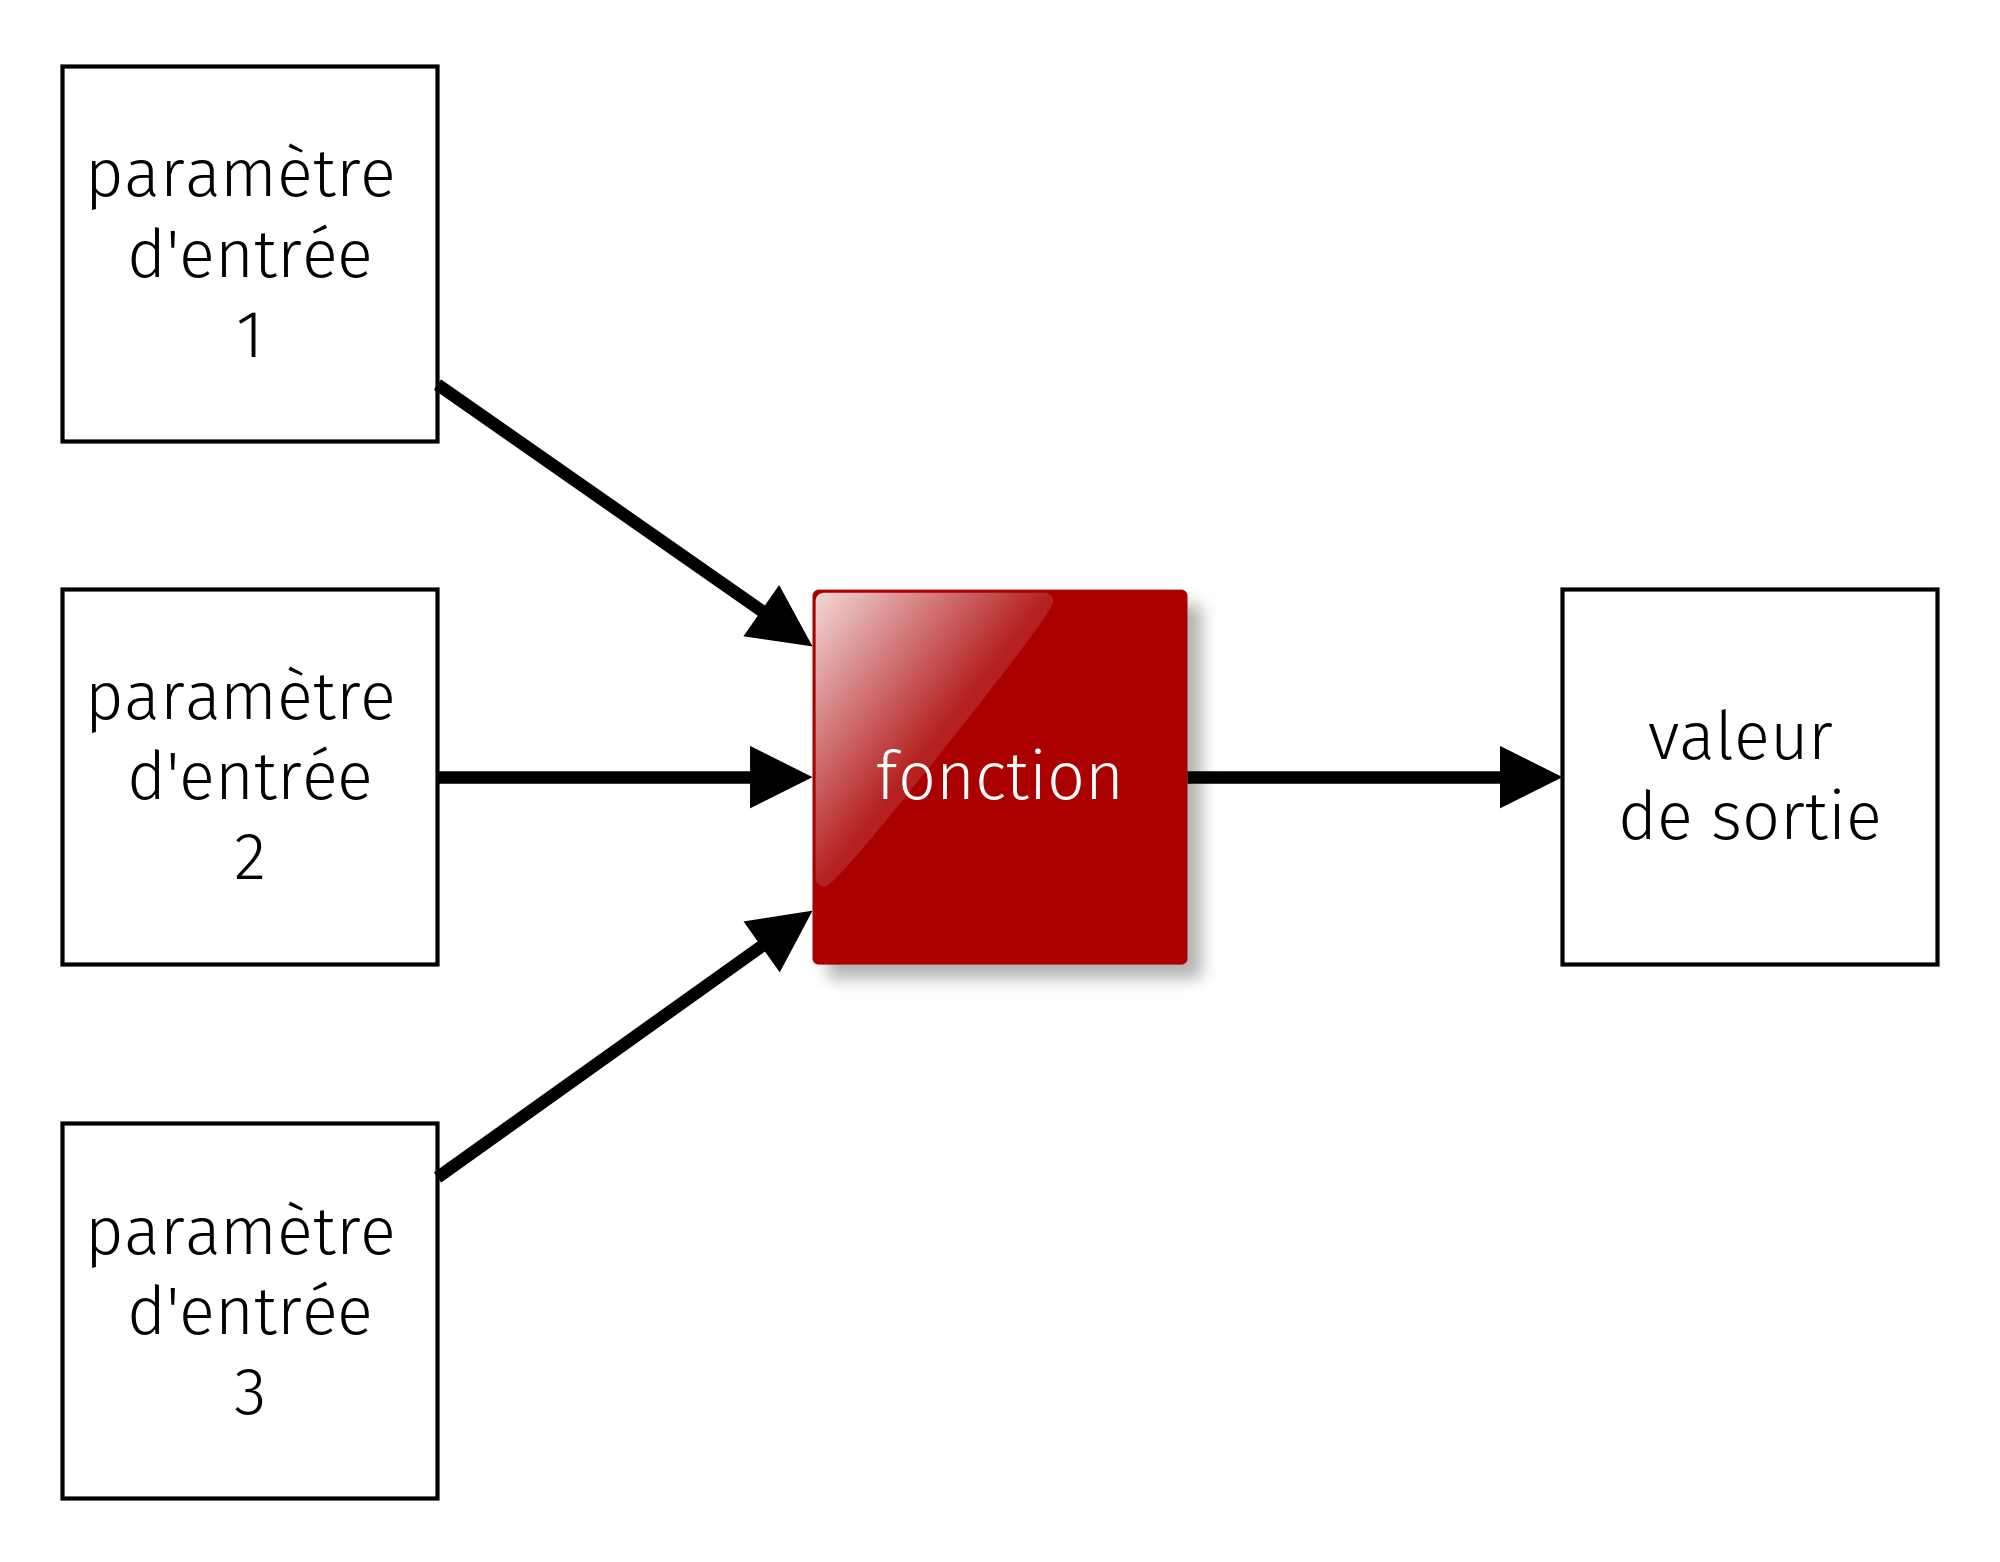
\includegraphics[width=6cm]{img/fonction2.png}
        \end{center}\pause
    Par exemple \mintinline{python}{max(20,3,10)} renvoie 20.
    \end{frame}
    \begin{frame}{De multiples formes}
        D'autres fonctions sont ainsi :
        \begin{center}
            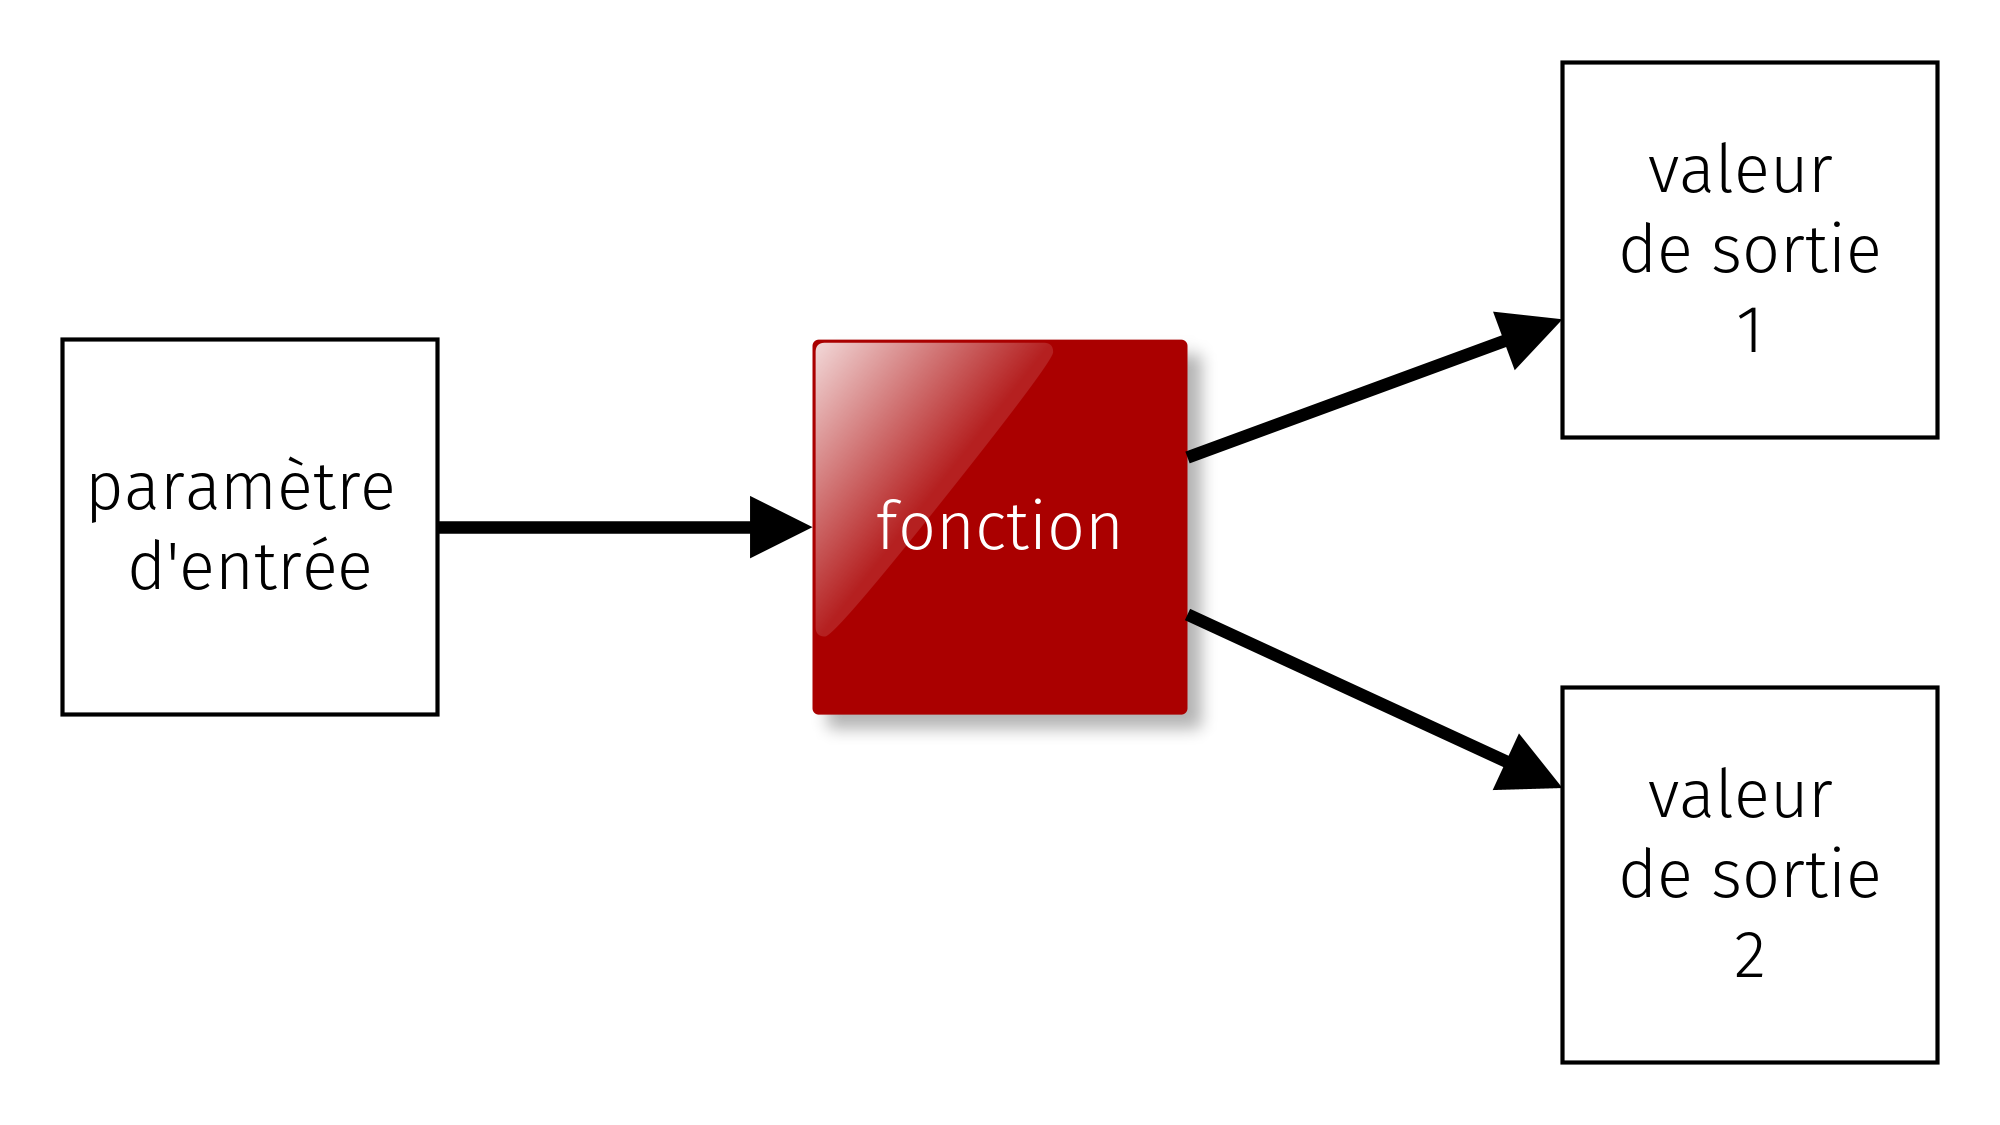
\includegraphics[width=6cm]{img/fonction3.png}
        \end{center}\pause
        On verra des exemples plus tard.
    \end{frame}
    \begin{frame}{De multiples formes}
        D'autres encore ainsi :
        \begin{center}
            
\includegraphics[width=6cm]{img/fonction4.png}
        \end{center}\pause
        Par exemple \mintinline{python}{print("salut")} ne renvoie rien mais affiche \mintinline{python}{salut} à l'écran.
    \end{frame}

    \begin{frame}{De multiples formes}
        D'autres suivent ce schéma :
        \begin{center}
            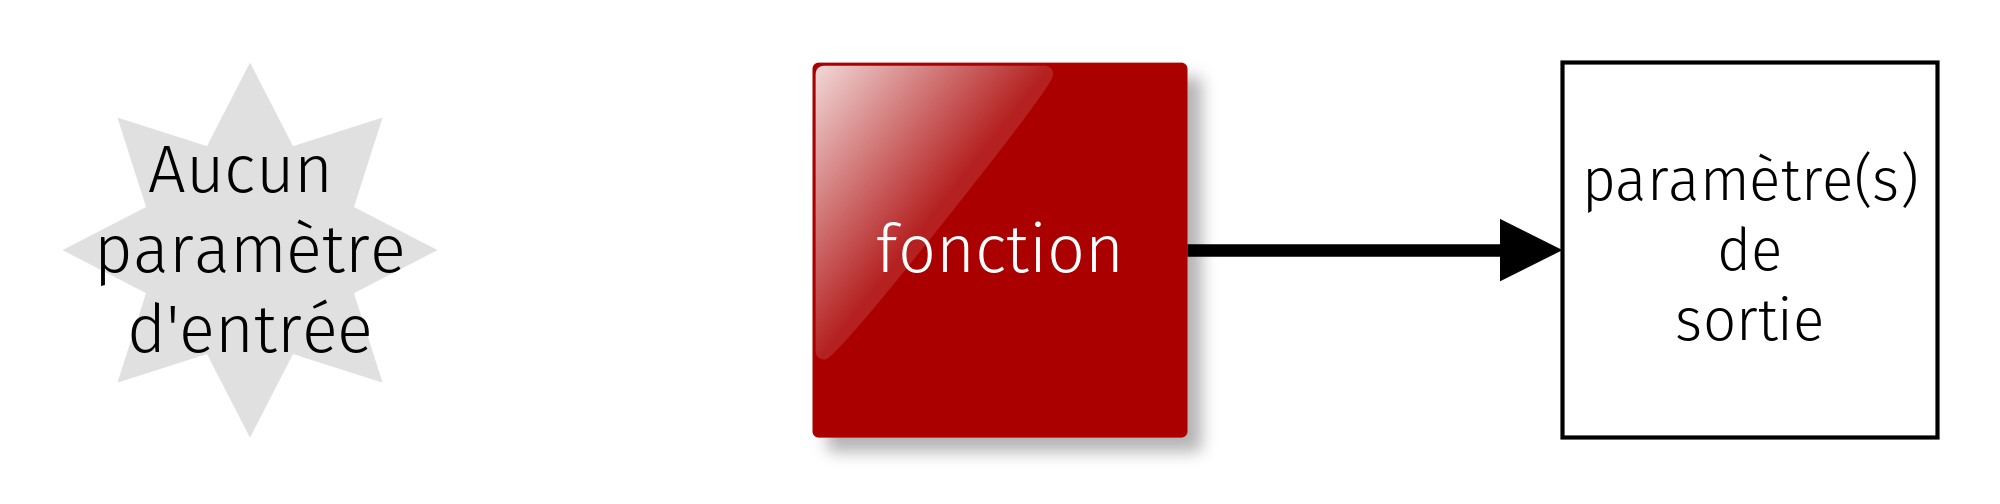
\includegraphics[width=6cm]{img/fonction5.png}
        \end{center}\pause
        Par exemple dans le module \mintinline{python}{time}, la fonction \mintinline{python}{time} ne prend aucun paramètre d'entrée mais renvoie l'heure qu'indique l'horloge de l'ordinateur.\pause\\
        On peut par exemple l'utiliser pour stocker une heure précise en tapant \mintinline{python}{maintenant = time()}.
    \end{frame}

    \begin{frame}{De multiples formes}
        Enfin certaines suivent ce schéma :
        \begin{center}
            
\includegraphics[width=6cm]{img/fonction6.png}
        \end{center}\pause
        Par exemple dans le module \mintinline{python}{p5}, \mintinline{python}{draw} ne prend aucun paramètre d'entrée, ne renvoie aucune valeur, mais actualise la fenêtre graphique.\pause
    \end{frame}
    \begin{frame}{Créer une fonction}
        Il est possible de créer de nouvelles fonctions.\\
        On parle à ce moment de fonctions \alert{côté concepteur}.\\

        Il faut donc définir rigoureusement ce qu'est une fonction.
    \end{frame}
    \section{Définition de la notion de fonction}
    \begin{frame}{Notion de fonction}
        \begin{block}{Définition}
            Une \textit{fonction} est un \og morceau de code\fg{} qui représente un \textit{sous-programme}.\\
            Elle a pour but d'effectuer une tâche \textit{de manière indépendante}.\\
        \end{block}
    \end{frame}
    \begin{frame}[fragile]{Un exemple}
        On veut modéliser la fonction mathématique $f$ définie pour tout nombre réel $x$ par $$f(x)=x^2+3x +2$$\pause

        On écrira alors

          \begin{minted}[breaklines,breakanywhere]{python}
def f(x : float) -> float:
    return x ** 2 + 3 * x + 2
            \end{minted}
 \pause
    Pour évaluer ce que vaut $f(10)$ et affecter cette valeur à une variable, on pourra désormais écrire \mintinline{python}{resultat = f(10)}.
    \end{frame}
    \begin{frame}[fragile]{Question}
        Que fait cette fonction \mintinline{python}{mystere} ?

            \begin{minted}[breaklines,breakanywhere]{python}
def mystere(a : float, b : float) -> float:
    if a <= b:
        return b
    else:
        return a
            \end{minted}
\pause
        La fonction \mintinline{python}{mystere}:
        \begin{itemize}
            \item	prend en entrée deux paramètres de type \mintinline{python}{float} \mintinline{python}{a} et \mintinline{python}{b}; \pause
            \item	renvoie le plus grand de ces deux nombres.
        \end{itemize}
    \end{frame}
    \begin{frame}{Spécification}
        La réponse que l'on vient de formuler s'appelle \textit{la spécification} de la fonction $f$.
    \end{frame}
    \begin{frame}{Spécification}
        \begin{block}{Définition}
            Donner la spécification d'une fonction \mintinline{python}{f} c'est\pause
            \begin{itemize}
                \item	préciser le(s) type(s) du (des) paramètre(s) d'entrée (s'il y en a);\pause
                \item	indiquer sommairement ce que fait la fonction \mintinline{python}{f};\pause
                \item 	préciser le(s) type(s) de la (des) valeur(s) de sortie (s'il y en a).
            \end{itemize}
        \end{block}
    \end{frame}
    \section{Anatomie d'une fonction}
    \begin{frame}[fragile]{Exemple}
            \inputminted{python}{scripts/min.py}\pause
        La fonction \mintinline{python}{f}
        \begin{itemize}
            \item	prend en entrée une liste (sous entendu d'entiers);\pause
            \item	renvoie le plus petit entier de cette liste.
        \end{itemize}
    \end{frame}
    \begin{frame}{Anatomie de la fonction : paramètre formel}
        \begin{center}
            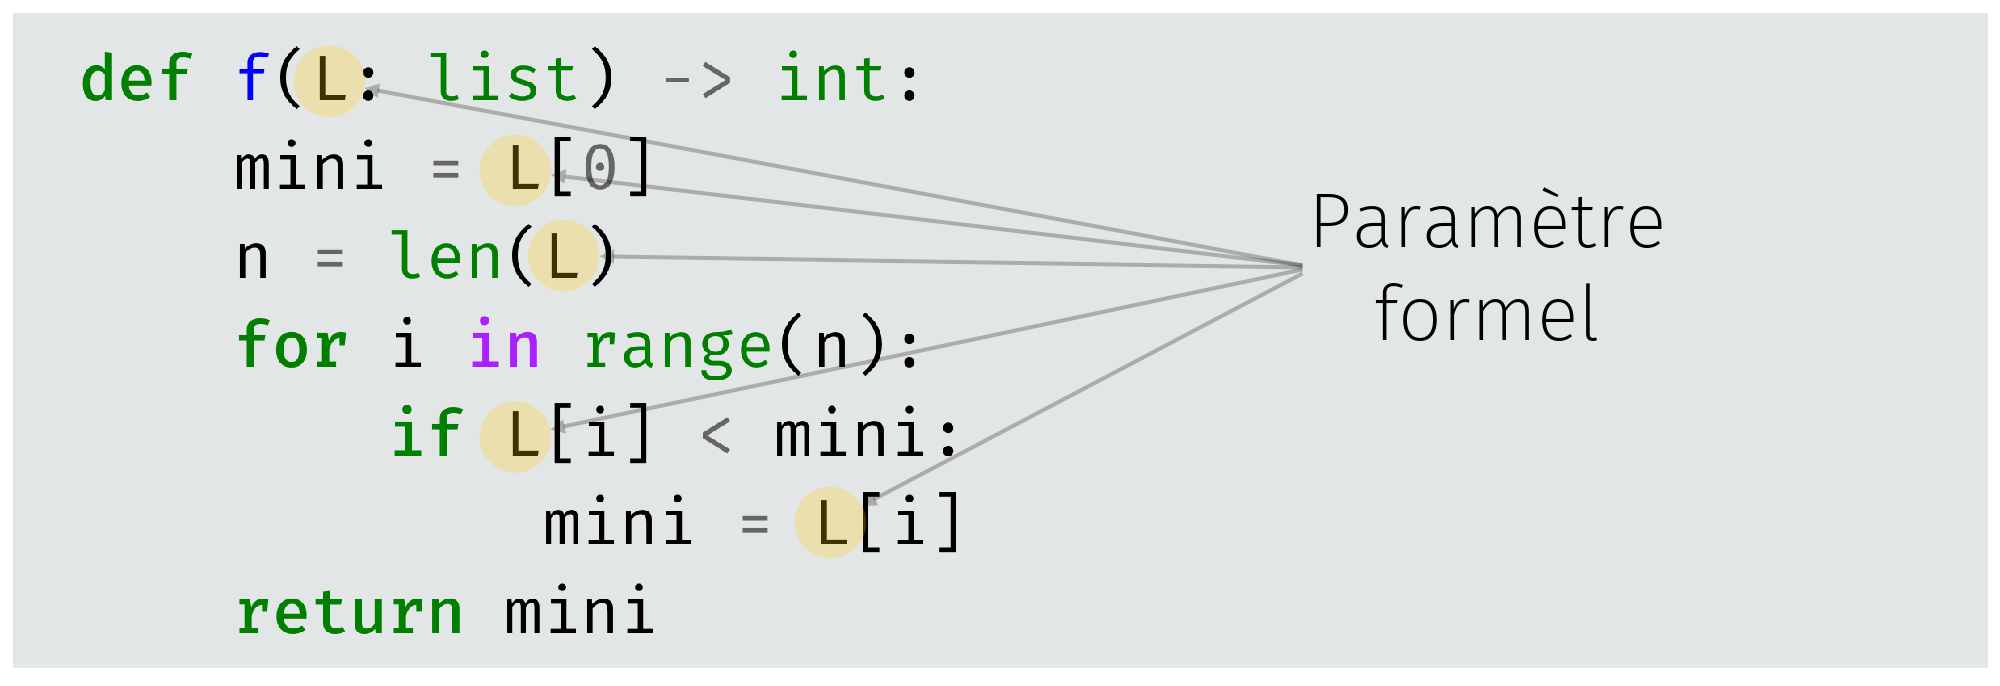
\includegraphics[width=11cm]{img/anat1}
        \end{center}\pause
    Le paramètre d'entrée est \textit{formel} : \alert{le nom de cette variable n'existe qu'à l'intérieur de la fonction}.\\\pause
    Si ce nom de variable existe déjà à l'extérieur de la fonction, \alert{ce n'est pas la même variable}.
    \end{frame}

    \begin{frame}{Anatomie de la fonction : paramètre formel}
    \begin{center}
        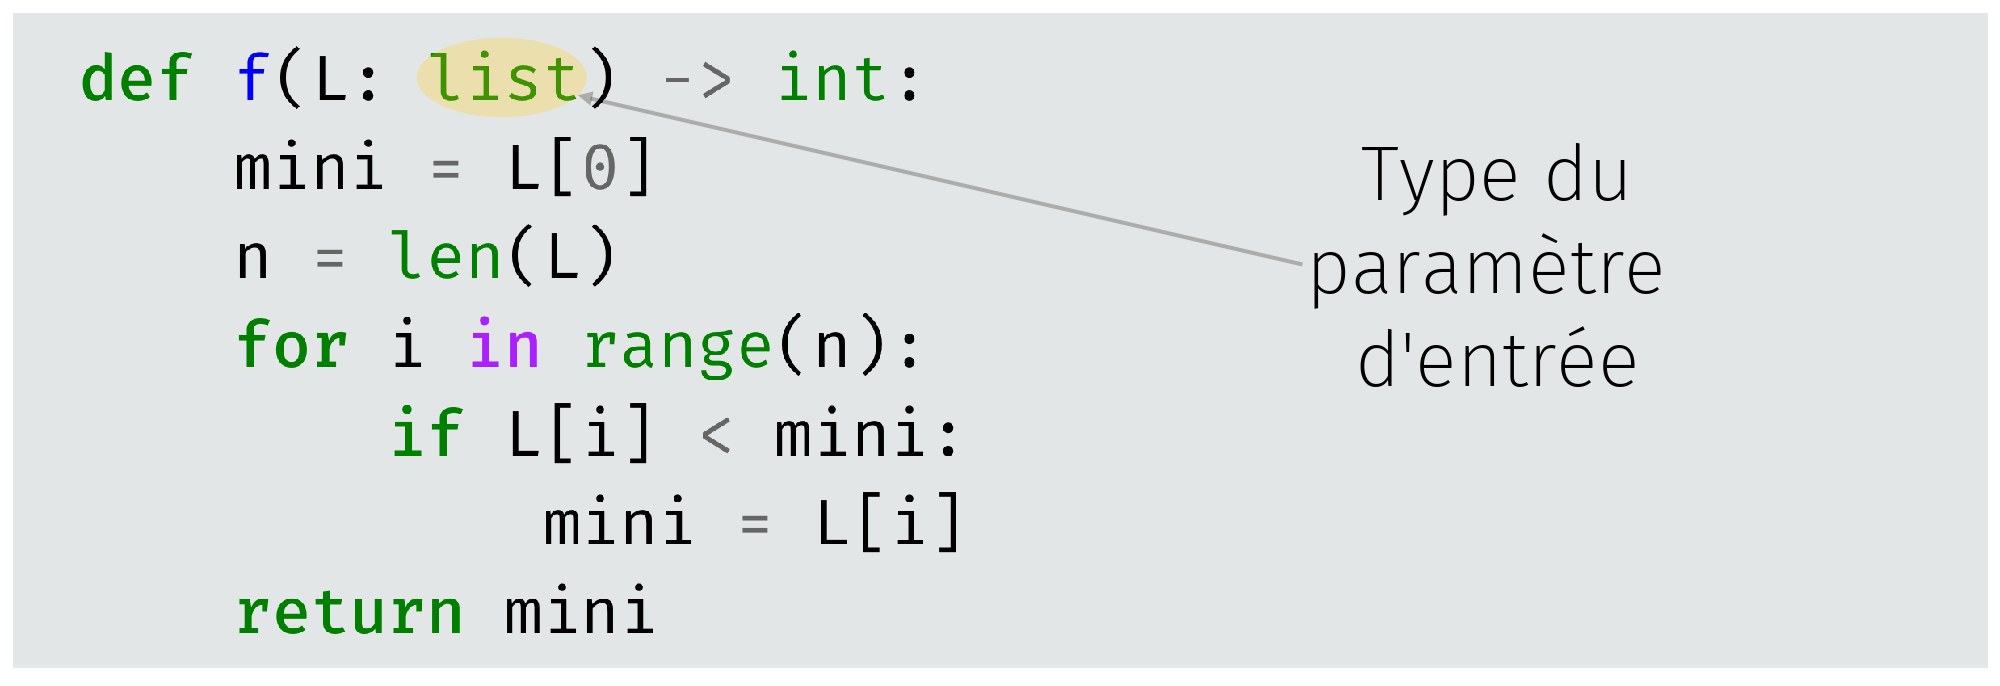
\includegraphics[width=11cm]{img/anat4}
    \end{center}\pause
    Le type du paramètre d'entrée peut être spécifié. Ce n'est pas obligatoire mais très fortement recommandé pour \og garder les idées claires\fg{}.
    \end{frame}
    \begin{frame}{Anatomie de la fonction : variables locales}
    \begin{center}
        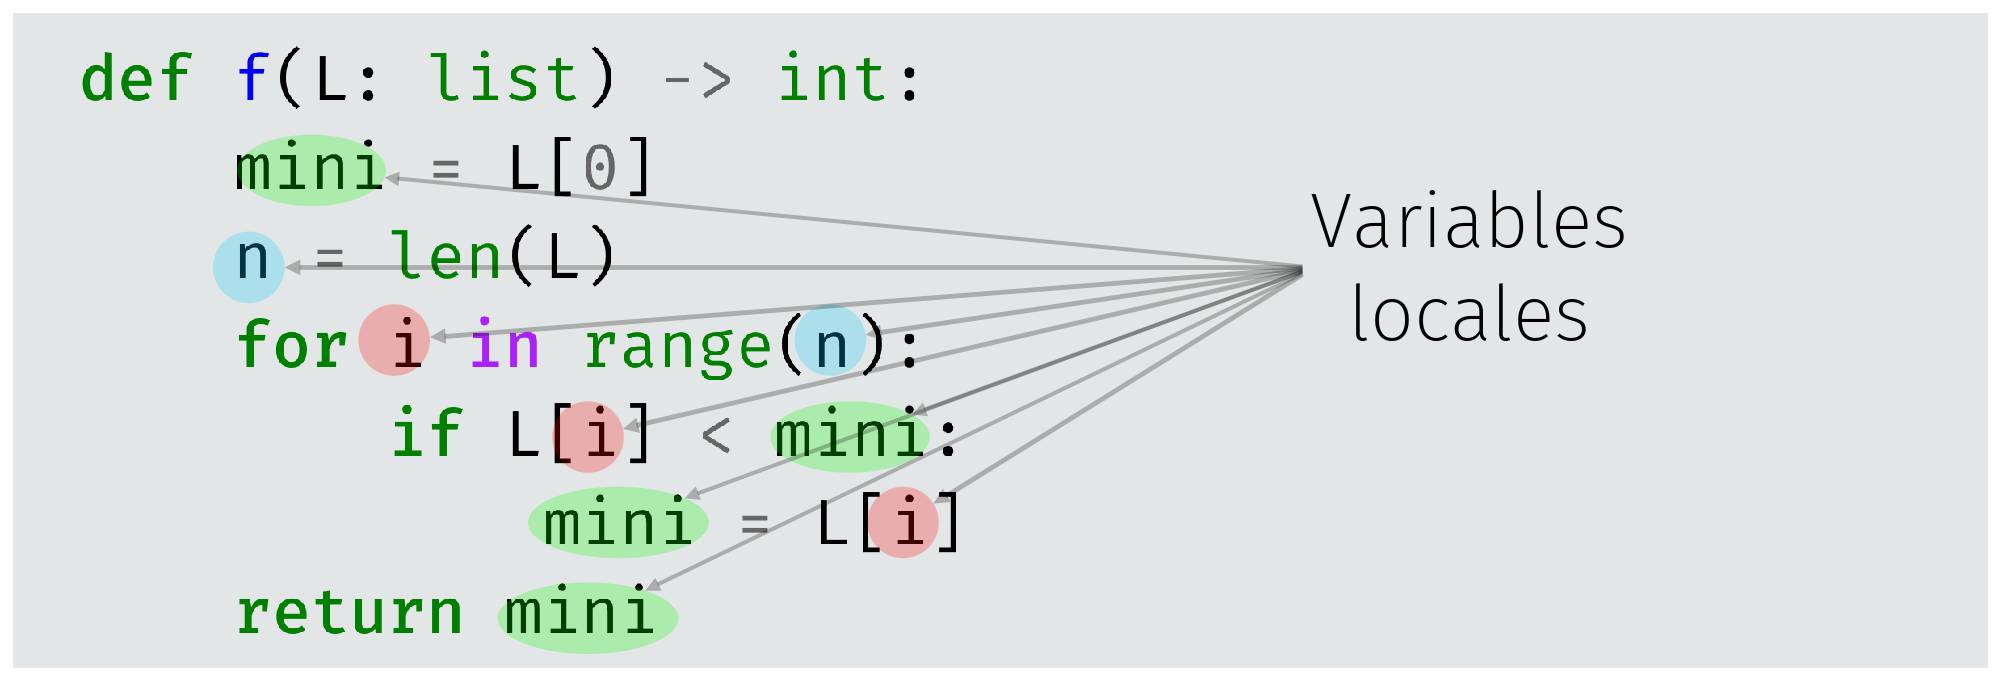
\includegraphics[width=11cm]{img/anat2}
    \end{center}\pause
    Toutes les variables \alert{créées} dans une fonction n'existent \alert{que dans cette fonction}.\pause Elles ne sont pas accessibles depuis l'extérieur de la fonction. On dit que ce sont des \alert{variables locales}.
    \end{frame}
    \begin{frame}{Anatomie de la fonction : valeur de sortie}
    \begin{center}
        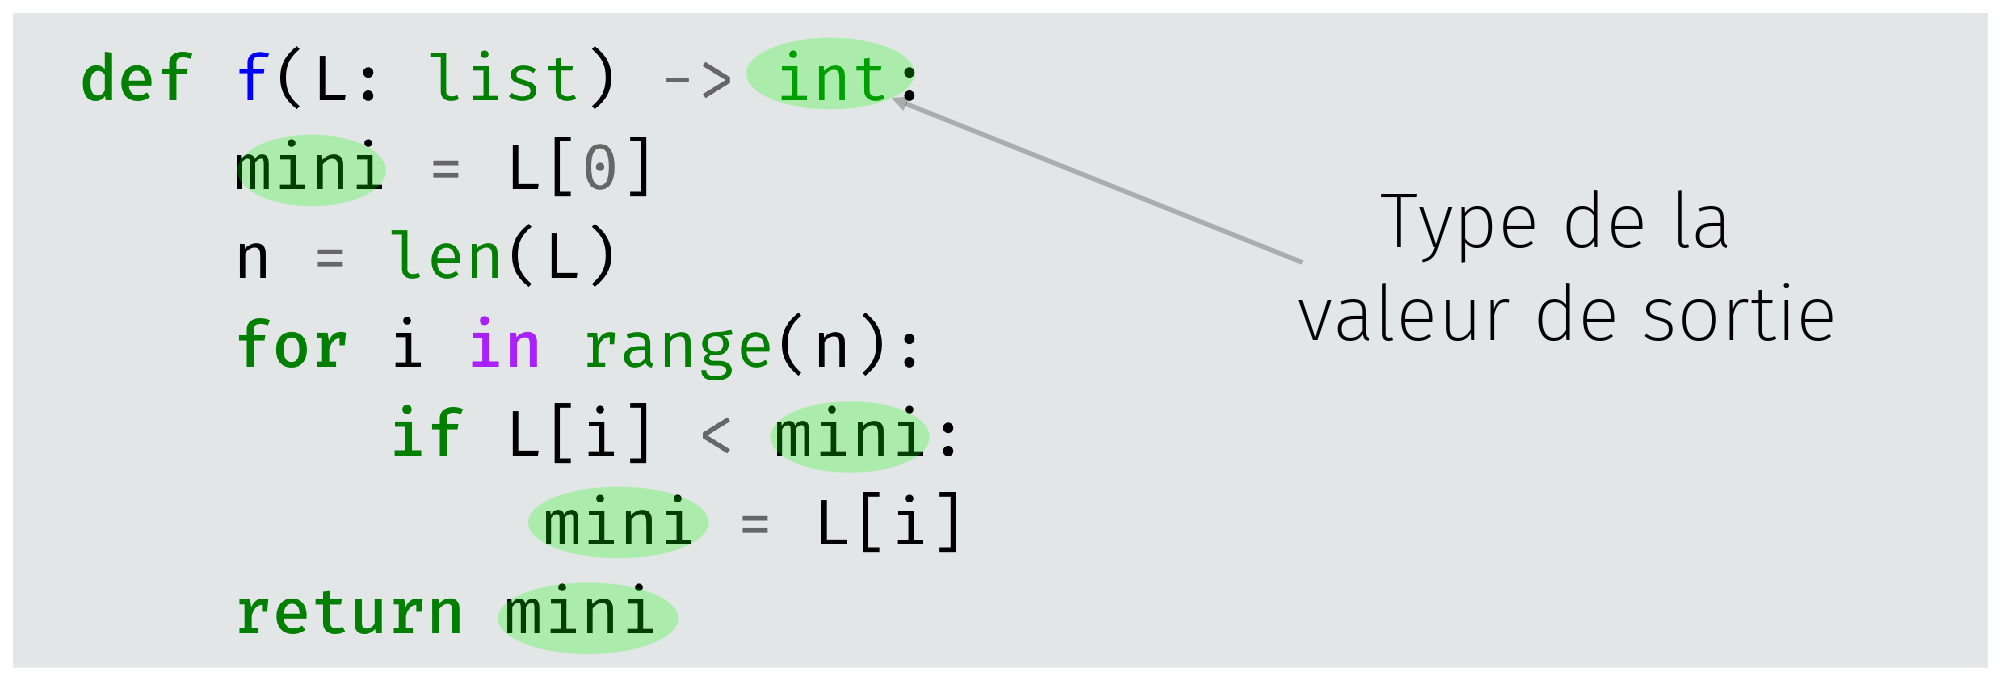
\includegraphics[width=11cm]{img/anat3}
    \end{center}\pause
    Le type de la valeur de sortie peut être précisé, c'est également recommandé.
\end{frame}
\section{En pratique}
\begin{frame}[fragile]{Chronologie}
    \begin{minted}[linenos]{python}
def f(x : float) -> float:
    return x ** 2 + 3 * x + 2

print(f(1)) # Affiche 6
    \end{minted}
    \pause
    Le programme commence à la ligne 4 !\\
    Les 2 premières lignes servent à définir la fonction \texttt{f}, elles ne sont exécutées que lorsqu'on évalue \texttt{f(1)}.
\end{frame}


\begin{frame}[fragile]{Exemple 1}
\begin{minted}{python}
def f(x : float) -> float:
    return x ** 2 + 3 * x + 2

print(x) # Provoque une erreur
\end{minted}
\pause
L'erreur vient du fait que la variable \texttt{x} \alert{n'est pas définie}. Le \og \texttt{x} qu'on voit dans la fonction \texttt{f}\fg{} est un paramètre formel et n'existe que dans \texttt{f}.
\end{frame}

\begin{frame}[fragile]{Exemple 2}
    \begin{minted}{python}
def f(x : float) -> float:
    a = 2
    return x + a

print(a) # Provoque une erreur
    \end{minted}
\pause
L'erreur vient du fait que la variable \texttt{a} \alert{est locale} : elle n'est définie que durant l'exécution de \texttt{f}.
\end{frame}
\begin{frame}[fragile]{Exemple 3}
    \begin{minted}{python}
def f(x : float) -> float:
    a = 2
    return x + a

print(f(4)) # Affiche 6
print(a) # Provoque une erreur
    \end{minted}
\pause
C'est encore la même erreur : une fois \texttt{f(4)} évaluée, \texttt{a} n'existe plus.
\end{frame}

\begin{frame}[fragile]{Exemple 4}
    \begin{minted}[linenos]{python}
def f(x : float) -> float:
    a = 2
    return x + a

a = 3
print(f(4)) # Affiche 6
print(a) # Affiche 3 et pas 2
\end{minted}
\pause

La variable \texttt{a} définie dans la fonction \texttt{f} n'est pas la même que celle qui est définie à la ligne 5.\\
Celle définie à la ligne 2 est \alert{locale}.\\
La variable \texttt{a} de la ligne 5 est appelée \alert{globale}.
\end{frame}


\begin{frame}[fragile]{Exemple 4}
\begin{minted}[linenos]{python}
def f(x : float) -> float:
    return x + a

a = 3
print(f(4)) # Affiche 7

\end{minted}
    \pause
\metroset{block=fill}
\begin{alertblock}{À retenir}
    Une fonction a le droit d'\alert{accéder en lecture} à une variable globale, mais n'a pas \textit{a priori} le droit d'en modifier la valeur.
\end{alertblock}
\end{frame}

\begin{frame}[fragile]{À éviter}
    \begin{minted}[linenos]{python}
def f(x : float) -> float:
    global a
    a = a + 1
    return x + a

a = 3
print(f(4)) # Affiche 8
print(a) # Affiche 4

\end{minted}
    \pause
À la ligne 2, on signale à Python que \texttt{f} a la droit de modifier la variable globale \texttt{a}.\\

C'est fortement déconseillé : sauf si on ne peut pas faire autrement, une fonction ne doit pas modifier les variables globales.

\end{frame}


\end{document}